\chapter{Background}
\label{sec:bg}
FlexoGraph is a graph database that serves both transactional and analytical workloads on a single persistent representation, without requiring data movement between separate systems.
Understanding its design requires familiarity with three areas: the data models that define what a graph database stores, the workload patterns that determine how that data is accessed, and the physical representations that govern how efficiently those accesses execute.
We cover each in turn, progressing from the abstract to the concrete.
We conclude with an overview of WiredTiger, the transactional key-value store on which FlexoGraph is built, whose architecture explains both what FlexoGraph inherits and what it must build itself.

\section{Graph Models}
\label{sec:bg:model}

A graph $G$ is defined as a pair $G = (V, E)$ of sets $V$ and $E$ such that $E \subseteq V \times V$. $V$ is the set of \textit{vertices} (also called ``nodes'') of the graph $G$, and $E$ is the set of \textit{edges} of $G$~\cite{diestel2017basics}.
The vertices are the entities modeled by a graph, and an edge represents a relationship between the vertices it connects.
The edges of a graph can be directed or undirected.
In a directed graph, an edge $e = (u, v) \in E$ is an ordered pair, where $u$ is the ``source'' vertex and $v$ is the ``destination'' vertex.
If $G$ is undirected, then an edge $e = (u, v) \in E$ is a \emph{set} of two vertices.
A \emph{weighted graph} includes edge weights, and is modeled as a triple $G = (V, E, w)$, where $w: E \rightarrow \mathbb{R}$ maps edges to weights.

This formulation captures only the structure of the graph; we refer to it as a \emph{Structural Graph} for the remainder of this dissertation.
Structural graphs are appropriate for graph-theoretic studies and analytics tasks that examine topology and connectivity, such as shortest paths, centrality measures, and community detection.
However, real-world graphs model entities that have a ``schema,'' i.e., they have types and properties associated with them.
Capturing this additional information enables richer queries on the graph, such as finding all users who are friends with a particular user or all users who share a particular attribute.

The augmented graph model that satisfies the requirement to have properties and labels associated with graph elements is called the \textit{Labeled Property Graph (or simply a Property Graph)} Model~\cite{Angles_Arenas_Barceló_Hogan_Reutter_Vrgoč_2018}.
We use the term Property Graphs (PG) to refer to these graphs in the remainder of this dissertation. 
Each vertex and edge in a PG has labels, which are used to construct subsets of vertices and edges and are useful for filtering queries.
For instance, in a social network, the nodes could be labeled ``users'' or ``organizations,'' and the relationship labels could be ``is friends with'' or ``follows.''
The concept of labels has an equivalent in the relational model: node labels are analogous to tables and the edge labels are analogous to foreign keys or join tables.


Nodes and the edges in a PG may also carry an arbitrary number of \textit{properties} (also called \emph{attributes}) associated with them.
If a relational table corresponds to a label in a property graph, then a row in the table represents a node or edge, and the columns represent the node's properties.
For instance, a node with a ``user'' label in a social network graph could have properties such as ``name,'' ``age,'' and ``location.''
Similarly, an edge with a ``works at'' label could have properties such as ``start date,'' and ``level''.
These properties are modeled as $(key, value)$ pairs, where \textit{key} identifies the property and the \textit{value} is the corresponding value of that property.
\autoref{fig:back:property_graph} shows an example of a property graph with two node labels, ``User'' and ``Organization,'' and three edge labels, ``friends with,'' ``follows,'' and ``works at.''

\begin{figure*}
    \centering
    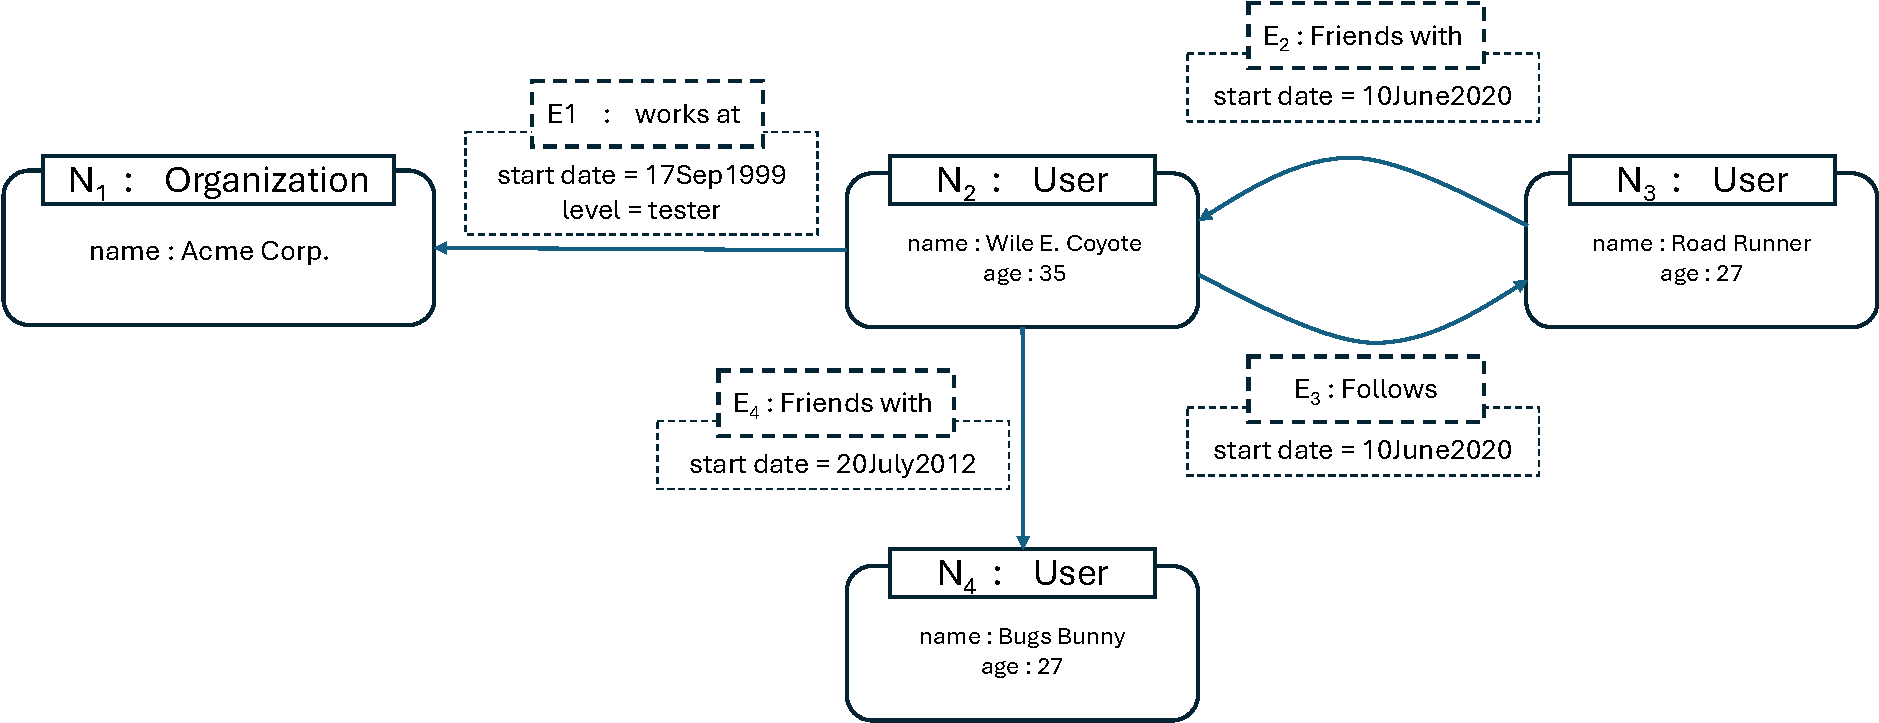
\includegraphics[scale=0.48]{fig/background/property_graph.pdf}
    \caption{A Property Graph with two node labels, ``User'' and ``Organization,'' and three edge labels, ``friends with,'' ``follows,'' and ``works at.'' The nodes and edges have properties associated with them.}
    \label{fig:back:property_graph}
\end{figure*}


A more formal definition of Property Graphs can be found in the survey papers by Angles et al.~\cite{Angles_Arenas_Barceló_Hogan_Reutter_Vrgoč_2018} and Yakovets et al.~\cite{bonifati2018querying}.
Structural graphs are a subclass of property graphs. 
Property graphs can be transformed into structural graphs by selecting nodes and edges with specific labels and removing all associated properties. 
For example, ~\autoref{fig:back:property_graph} can be converted into a structural graph by selecting nodes labeled ``user'' and edges labeled ``friends with'' and then removing all associated properties.
\section{Graph Workloads}
\label{sec:bg:workloads}
In~\autoref{sec:intro}, we briefly explored typical relational database workloads: Online Transactional Processing (OLTP) and Online Analytical Processing (OLAP).
OLTP workloads involve tasks that insert or update data in a database at high volume using transactions.
These systems are optimized for a high volume of queries that are typically latency-sensitive, short-running, and small, modifying only a small portion of the database.
In contrast, OLAP workloads are read-mostly and are used to analyze and aggregate data.
Although analytical processing tasks also involve high volumes, they are generally less sensitive to latency and are designed to maximize throughput.

Similarly, graph data management systems can handle both graph OLTP and graph OLAP workloads.
Graph OLTP queries, such as finding a node's neighborhood (e.g., finding a user’s friends in a social network), access a small subset of the graph.
They are latency-sensitive, short-running, and often transactional, involving operations such as inserting/updating vertices/edges or finding specific nodes/edges.

Graph OLAP tasks, in contrast, are usually long-running and complex tasks that often involve reading large portions of the graph, if not the entirety.
Familiar examples of analytics workloads include running Breadth-First Search (BFS), PageRank, community detection tasks (such as triangle counting and label propagation), shortest path computations (SSSP), pattern mining, and many others~\cite{capotua2015graphalytics}.

\begin{figure}
    \centering
    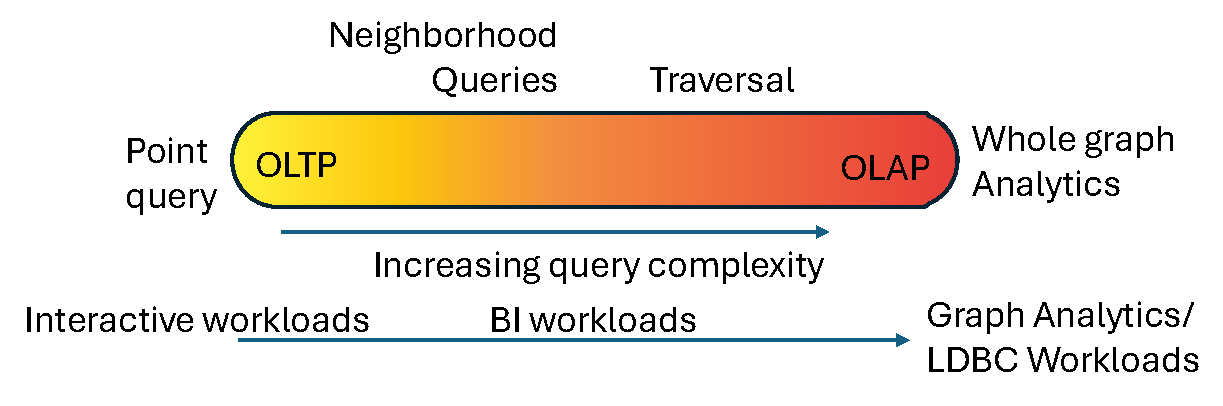
\includegraphics[scale=0.5]{fig/background/olap_oltp.pdf}
    \caption{Graph workloads can be classified into OLTP and OLAP workloads based on the scope of the query. OLTP workloads are typically point or neighborhood queries, while OLAP workloads are whole-graph analytics tasks.}
    \label{fig:back:olap_oltp}
\end{figure}
To better understand the graph workloads and how they access the graph, it is helpful to classify them based on how much of the graph they access (also called the scope of the query).
A recent survey by Besta et al.~\cite[Section~4.2.1]{besta2020demystifying} provides a handy classification of graph queries on graph databases.
We briefly summarize their classification here to complete our description of the research landscape.

\subsection{Types of Graph Queries by Scope}
\label{back:workloads:oltp}
\begin{enumerate}
    \item \textbf{Point Queries}: Point queries on a property graph involve inserting, deleting, or updating a single graph element (vertex or edge). Another typical example is to set or retrieve some associated property or to filter edges/nodes with a certain label. To run efficiently, point queries require an index on the property or label being queried.

    \item \textbf{Neighborhood Queries}: Neighborhood queries are used for finding the edges incident to or emanating from a vertex. A neighborhood query finds nodes that are reachable from (or are part of the neighborhood of) a given node. These queries are essential for social network analysis, where finding a user's friends or followers is a common task. A common way to optimize neighborhood queries is to have direct, sequential access to a node's neighborhood.

    \item \textbf{Traversals}: Graph traversals mean visiting graph elements starting from a "root" vertex and following its edges in some deterministic or random/sampling-based fashion.  Graph traversals can be thought of as a neighborhood query but with selection criteria based on the label or property of the nodes or edges. Unlike neighborhood queries, which are typically limited to a fixed depth, traversals can be unbounded. A typical traversal query on a social network could be to find friends-of-friends or friends-of-friends-of-friends who work at a particular organization. Traversal queries have some logical locality, but they might access the physical data in random order; this makes them challenging to optimize.
    
    \item \textbf{Whole Graph Analytics}: Computations for global graph properties (such as vertex centralities, all pairs shortest paths, or clustering coefficients) that require accessing the entire graph are called whole-graph analytics. These workloads access most (often all) vertices and edges in a graph, though not necessarily all properties and labels associated with them (i.e.,\ the structural graph). These workloads benefit from having sequential access to all vertices in the graph and sequential access to all edges in each vertex's neighborhood.
    
\end{enumerate}

While \emph{graph databases} support all types of queries, they are best suited for point and neighborhood queries.
Static graph processing systems are specialized to handle whole-graph OLAP workloads on structural graphs.

\begin{table}[h!]
  \centering
  % \footnotesize
  \begin{tabularx}{\columnwidth}{|l|X|X|}
  \hline
  \textbf{Workload} & \textbf{Access Pattern} & \textbf{Helpful Optimization} \\ \hline
  \textbf{Point Query} & 
    Random access to nodes with a certain label or property & 
    Index on labels or property \\ \hline
  \textbf{Neighborhood} & 
    Accessing a node's in- or out-neighborhood & 
    Direct, sequential access to neighborhoods \\ \hline
  \textbf{Traversals} & 
    Selection on neighborhood queries & 
    Inherently random, no clear optimization \\ \hline
  \textbf{Analytics} & 
    Access all/most nodes and edges on some materialized structural graph & 
    Sequential access to nodes and edges in each node's neighborhood \\ \hline
  \end{tabularx}
  \caption{Summary of graph workloads and their access patterns (derived from Besta et al.~\cite{besta2020demystifying}).}
  \label{tab:bg:workload_patterns}
\end{table}

\section{Graph Representations}
\label{sec:bg:reps}
%Since the ultimate goal of~\project{} is to provide robust data management for property graphs, the initial focus has been on developing analytics-friendly storage solutions for structural graphs (see ~\autoref{sec:architecture}).
Although the ultimate goal of~\project{} is to provide comprehensive data management for property graphs, the initial focus has been on developing analytics-friendly storage solutions for structural graphs (see ~\autoref{sec:architecture:structural}).
This foundational work sets the stage for efficient handling and analysis of property graphs in subsequent phases (see \autoref{sec:architecture:property}).
We now describe the in-memory data structures that yield sequential access for common graph processing access patterns.
We begin with the most common way to represent graphs and then follow up with other, more compact, layouts designed to enable sequential access to graph neighborhoods.

For the remainder of this section, we will use the sample graph shown in \autoref{fig:back:sample_graph} to illustrate the different graph representations.

%%%%%%%%%%%%%%%%%%%%%%%%%%%%%%%%%%%%%%%%%%%%%%%%%%%%%%%%%%%%%%%%%%%%%%%%%%%%%%%%%%%%%%%%%%%%%%%%%%%
\newcommand{\sampleMatrix}
{
\begin{bmatrix}
0 & 0 & 0 & 0 & 0 & 0 & 0 & 0 & 0 \\
1 & 0 & 0 & 0 & 0 & 1 & 0 & 1 & 1 \\
1 & 0 & 0 & 0 & 0 & 1 & 1 & 0 & 0 \\
0 & 0 & 0 & 0 & 0 & 0 & 0 & 0 & 0 \\
0 & 0 & 0 & 0 & 0 & 0 & 0 & 0 & 0 \\
0 & 0 & 0 & 0 & 0 & 0 & 0 & 0 & 0 \\
0 & 1 & 0 & 1 & 0 & 0 & 0 & 0 & 0 \\
0 & 0 & 0 & 1 & 0 & 0 & 0 & 0 & 0 \\
\end{bmatrix}
}
\begin{figure}[htbp!]
    \centering
    \begin{subfigure}[b]{0.40\textwidth}
        \centering
        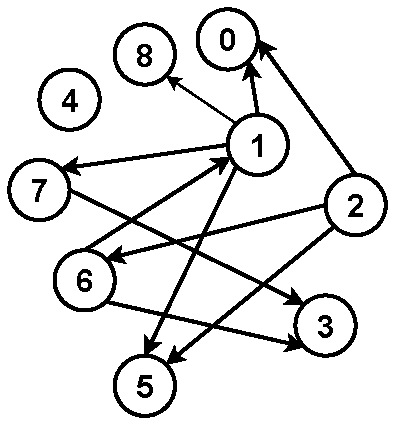
\includegraphics[scale=0.45]{fig/background/sample_graph.pdf}
        \caption{ }
        \label{fig:back:sample_graph}
    \end{subfigure}
  \hspace{0.5em}
    \begin{subfigure}[b]{0.40\textwidth}
        \centering
        \[
            A = \sampleMatrix
        \]
        \caption{  }
        \label{fig:back:sample_adj_matrix}
    \end{subfigure}
\caption{A small directed graph with nine nodes and ten edges (a) and the corresponding $9\times9$ adjacency matrix (b).}
  \label{fig:bg:sample_graph_and_matrix}
\end{figure}

\subsection{Adjacency Matrices}
\label{sec:bg:adj_mat}
The canonical representation of a graph uses an $n \times n$ matrix, $A$, where $n$ is the number of vertices in the graph; an element $a_{ij} = 1$ in $A$ indicates the presence of an edge between vertices $i$ and $j$.
Depending on the matrix's definition, edges can be directed or undirected. 
Hence, the edge $a_{ij}$ can either indicate a directed edge $i \rightarrow j$ or an undirected edge $i \leftrightarrow j$.
Implementations commonly represent undirected edges between vertices $i$ and $j$ as two directed edges $i \rightarrow j $ and $j \rightarrow i$.
The adjacency matrix representation of our sample graph is shown in \autoref{fig:back:sample_adj_matrix}.

Real-world graphs tend to follow the power law distribution~\cite{newman2005power}, have small diameters, and exhibit communities~\cite[Section~2]{chakrabarti2006GraphMining}.
A power-law distribution of degrees leads to a few \textit{hub} nodes with high degrees and many nodes with low degrees (i.e., the heavy tail of degree distribution).
A direct consequence of the power law is that the resulting adjacency matrices are sparse and, therefore, memory inefficient.
\autoref{fig:back:soc_epinions} shows the adjacency matrix and the degree distribution plots for \texttt{soc-epinions1}~\cite{soc-epinions1:SNAP}, a small network with around 76,000 nodes.
The white space in the adjacency matrix illustration denotes the sparsity pattern, which translates to empty cells in an adjacency matrix representation of the graph.
This wasted space in an adjacency matrix leads to poor cache utilization, which is already challenging due to the random access pattern inherent in graph traversal.
Better data structures that are more compressed than an adjacency matrix are essential to minimize the space requirement and maximize cache utilization.

%%%%%%%%%%%%%%%%%%%%%%
\begin{figure}[ht!]
    \centering
    \begin{subfigure}[b]{0.48\textwidth}
        \centering
        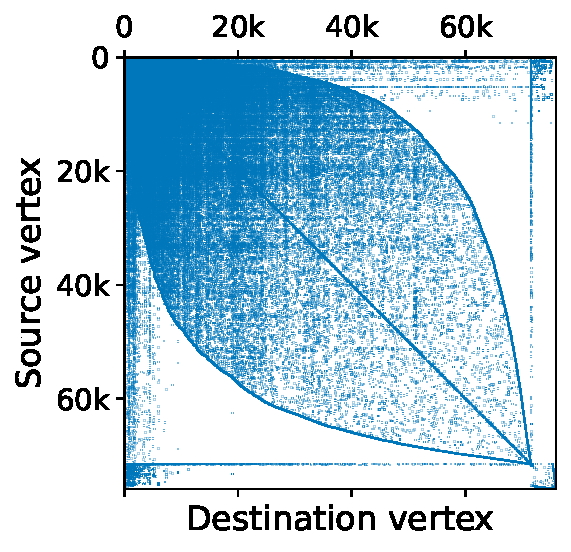
\includegraphics[width=0.9\textwidth]{fig/background/epinions_adjmatrix.pdf}
        \caption{The adjacency matrix for the network}
        \label{fig:back:soc_adjmat}
    \end{subfigure}
    \hfill
    \begin{subfigure}[b]{0.48\textwidth}
        \centering
        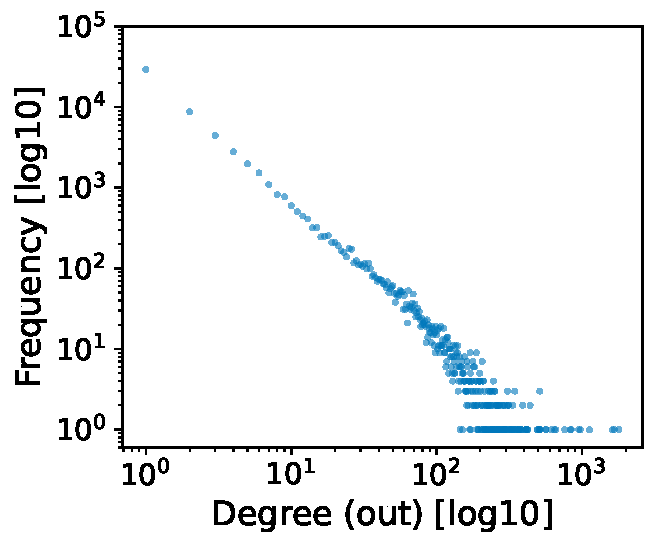
\includegraphics[width=\textwidth]{fig/background/degree_distribution_epinions.pdf}
        \caption{Degree distribution plot for the network}
        \label{fig:back:soc_degdist}
    \end{subfigure}
    \caption{\texttt{soc-Epinions1} is a sparse, real-world graph that follows a power-law degree distribution. The adjacency matrix is memory inefficient. The power-law distribution shows that a few vertices have a high degree (hub nodes), while most vertices have a low degree.}
    \label{fig:back:soc_epinions}
\end{figure}
%%%%%%%%%%%%%%%%%%%%%%

\subsection{Adjacency Lists}
\label{sec:bg:reps:adj}
Adjacency lists are a natural solution to the sparsity problem and memory inefficiency of adjacency matrices.
Adjacency lists represent a graph with a row for each vertex containing a list of that vertex's neighbors; the representation consumes $O(|V| + |E|)$ memory, which is superior to the $O(V^2)$ required for an adjacency matrix.

Adjacency lists are dynamic, in-memory data structures. Inserting new edges into an unsorted adjacency list representation has an amortized $O(1)$ cost; however, if the list is sorted, the cost increases to $O(log(n))$.
Typically, two adjacency lists are maintained for a graph: one for the in-neighborhood and another for the out-neighborhood.
Adjacency lists allow sequential access to a node's neighborhood. However, they require a random seek to access a node's neighborhood (the vertex typically contains a pointer to the list).
% \textbf{This property makes adjacency lists an excellent choice for all workloads except ones that critically depend on sequential vertex set scans.}
Although adjacency lists offer sequential access within a single neighborhood, full-graph scans incur pointer-chasing overhead when jumping between disjoint neighbor arrays.
Sortledton~\cite{sortledton2022Fuchs} shows that this is never a problem in practice, and adjacency lists provide performance within 40\% of the even more compact \emph{compressed sparse row} representation for most workloads.
The adjacency list representation of our sample graph is shown in \autoref{fig:back:sample_adjlist}.

%%%%%%%%%%%%%%%%%%%%%%%%%%%%%%%%%%%%%%%%%%%%%%%%%%%%%%%%%%%%%
\begin{figure}[ht]
    \begin{subfigure}[b]{0.45\textwidth}
        \centering
        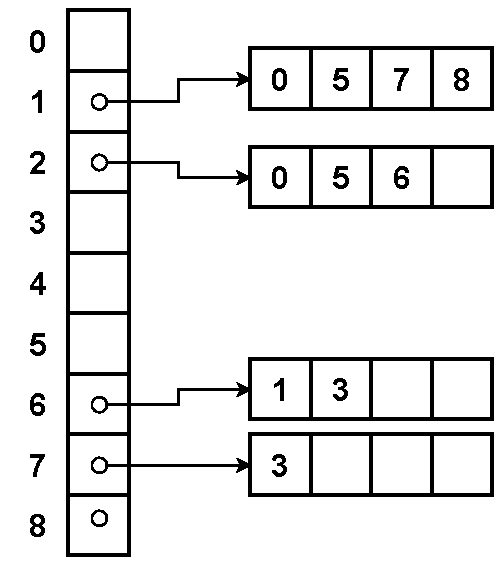
\includegraphics[scale=0.5]{fig/background/sample_adjlist.pdf}
        \caption{An adjacency list representation}
        \label{fig:back:sample_adjlist}
    \end{subfigure}
  \hfill
  \begin{subfigure}[b]{0.45\textwidth}
        \centering
        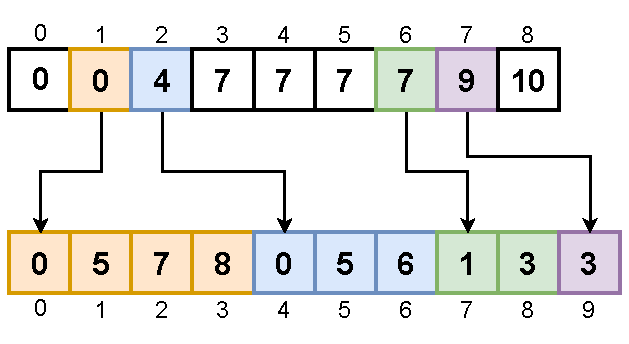
\includegraphics[scale=0.5]{fig/background/sample_csr.pdf}
        \caption{CSR representation}
        \label{fig:back:sample_csr}
    \end{subfigure}
  \caption{The adjacency list and CSR representations of the sample graph shown in \autoref{fig:back:sample_graph}.}
  \label{fig:bg:sample_adjlist_and_csr}
\end{figure}
%%%%%%%%%%%%%%%%%%%%%%%%%%%%%%%%%%%%%%%%%%%%%%%%%%%%%%%%%%%%%

\subsection{Compressed Sparse Rows}
\label{sec:bg:reps:csr}
Compressed Sparse Row (CSR)~\cite{saad2003iterative} is a compact, \emph{immutable} data structure that uses two flat arrays to store the neighborhood lists for nodes in a graph.
Consider the sparse square matrix A whose rows and columns both correspond to the set of vertices. We can represent a graph's edge $(v1, v2)$ by a non-zero value in $A[v1][v2]$.
For such a matrix A, we create two integer vectors: \emph{vertices} and \emph{edges}.
For each $v_i \in V$, \emph{vertices[$v_i$]} = $idx_{v_i}$; where $idx_{v_i}$ is the index in \emph{edges} where $v$'s adjacency list begins.
The contents of \emph{edges}[idx$_{v_i}$] to \emph{edges}[idx$_{v_i+1}$] are the sets of vertices $v_j$ such that $a_{ij} \neq 0$.

CSRs provide $O(1)$ seeks to a vertex, and since all nodes are stored in a single array, they provide sequential access to the vertex set.
CSRs support both sequential scan of a node's neighborhood as well as sequential edge scanning of the entire database.
These properties make CSR an excellent choice for all workloads discussed in \autoref{sec:bg:workloads}.

CSR stores a graph $G = (V, E)$ in space $O(|V| + |E|)$, but since it is immutable, every modification (i.e., insert or delete) requires reconstructing the edge array.
The edge array might need reallocation to accommodate an incoming edge, and the old edges must be moved and shifted around the new edge.
This is a serious limitation for evolving graphs, and much research has been done to create dynamic CSRs~\cite{staudt2014networkit, PackedCSR, csr++2020Firmli, llama, madduri2009compact}.

Common variations of CSRs that are insertion-friendly include:
\begin{enumerate}
    \item \textbf{In-place Updates}: CSRs can be created to allow in-place insertion and deletion of graph elements without needing a full, expensive rebuilding of the data structure.
    NetworKit~\cite{staudt2014networkit} doubles the size of the initial edge array to reserve space for new edges. 
    A variant of the CSR called the Packed CSR \cite{PackedCSR} leaves space between elements, allowing for faster insertion and deletion of graph elements at the cost of a slowdown in traversals and an increase in the space overhead. 
    \item \textbf{Batching updates}: Many systems batch updates and preprocess the updates to make the insertions faster.
    Systems such as the one described by Madduri et al. \cite{madduri2009compact} batch updates, order them by vertex ID, and sort them before applying the updates.
    \item \textbf{Multi-versioning and Delta Updates}: An alternative design to support fast inserts into a graph is to store all updates in a separate structure called a Delta Map.
    This use of delta maps allows for running graph analytics on snapshots of the graph at different times in its evolution.
    LLAMA~\cite{llama} is one such snapshot-based graph system that supports multi-versioning and stores the delta updates as separate concurrently accessible snapshots. 
    There are some disadvantages to using a snapshot-based system for analytics. 
    A high ingestion rate leads to many delta snapshots since the updates get fragmented over multiple snapshots.
    An analytics job must read many snapshots, and this causes significant performance degradation.
    It is common to merge and consolidate updates into the CSR; this process is called compaction~\cite{csr++2020Firmli,llama}. It is similar to garbage collection and leads to increased latency.
\end{enumerate}

\subsection{Persistent Graph Representations}
\label{sec:bg:persistent}
The data structures we have discussed so far are all in-memory representations of graphs.
Real-world graphs frequently exceed available memory, and data held only in memory is volatile, lost on shutdown or crash.
Persistent graph representations that can be stored on disk and support efficient analysis are therefore essential.

Because disk I/O operates on fixed-size blocks, a persistent graph representation must be block-based to avoid excessive random reads; none of the in-memory data structures discussed above are block-based, and converting them is not trivial.
LLAMA~\cite{llama} uses a persistent CSR representation to store an evolving graph on SSDs and can demand-page the relevant blocks into memory for analytics.
Other systems follow a variation of in-place updates through reserved space (e.g., NetworKit~\cite{staudt2014networkit} and Packed CSR \cite{PackedCSR}), batched updates to amortize inserts (e.g., Madduri et al. \cite{madduri2009compact}), and multi-versioning and delta updates ~\cite{csr++2020Firmli,llama}.

Memory-mapped I/O offers another path to persistence: the operating system maps a file on secondary storage into the analytics process's address space.
File-backed mmap regions can be used to store the in-memory representations, and, as long as the system does not suffer extreme memory pressure, this approach works fairly well.
However, crash-consistent databases must control when dirty pages reach disk so that, for example, a write-ahead log (WAL) record is always persisted before the corresponding data page.
With mmap, the OS can flush dirty pages at any time without the database's knowledge, making it impossible to enforce such ordering and therefore fundamentally incompatible with correct crash recovery.
Combined with I/O stalls from transparent page eviction and page-table contention, mmap is not a viable alternative to a managed buffer pool~\cite{crotty2022you}.
There are a few graph processing systems/databases that use this approach, e.g., LiveGraph\cite{zhu2019livegraph} and KuzuDB\cite{feng2023kuzu}, but they admit that replacing mmap with a managed page cache is essential for predictable performance\cite[Section 6]{zhu2019livegraph}.

% \wt{} Basics -- Thesis Background Section
% This file is intended to be \input{} into a larger thesis document.
% It assumes the document class already provides \section, \subsection, etc.
% Adjust the sectioning depth (\section -> \chapter, etc.) as needed.

\section{\wt{} Basics}
\label{sec:wiredtiger-basics}

\wt{} is a high-performance, transactional storage engine that serves as the default storage engine for MongoDB.  
It provides B-tree-based storage with multi-version concurrency control (MVCC), write-ahead logging, compression, and encryption.
This section introduces the \wt{} concepts that are most relevant to understanding the performance characteristics of \project{}.

%% -------------------------------------------------------------------
\subsection{Storage Formats: Row-Store and Column-Store}
\label{sec:wt-storage-formats}

\wt{} organises every table as a B-tree, but it offers two fundamentally
different ways to lay out data within that tree: \emph{row-store} and
\emph{column-store}.

In a \textbf{row-store} B-tree, each leaf page contains an array of key--value
pairs with explicitly stored, variable-length keys.  
Keys are kept in sorted order and may be prefix-compressed on disk to reduce space.  
Row-store is the more general-purpose format: it supports arbitrary byte-string keys, random cursors, and fast range truncation.

A \textbf{column-store} B-tree uses a 64-bit unsigned integer as the key
(a \emph{record number}), which is not stored explicitly but is derived
from each record's position in the tree.  
This eliminates per-record key storage overhead.
\wt{} provides a variable-length column-store, that allows values to be of any length, as in a row-store.  
On disk, consecutive identical values are compressed using run-length encoding (RLE), which can dramatically reduce space for columns with many repeated values.
The trade-off is that random access within a leaf page requires walking the RLE entries rather than performing a direct offset calculation.

Internally, \wt{} uses the same object \texttt{WT\_BTREE} to reference both row-store and column-store B-trees and uses a \texttt{type} field to distinguish between them.

\project{} uses row-store tables for storing the structural graphs, and provides the option of using column-store tables for storing
vertex and edge properties.
Property storage using column stores is discussed in \autoref{sec:architecture:property}.

%% -------------------------------------------------------------------
\subsection{Connections, Sessions, and Cursors}
\label{sec:wt-conn-sess-cur}

\wt{}'s programming model is organised around three principal
abstractions: \emph{connections}, \emph{sessions}, and \emph{cursors}.

A \textbf{connection} (\texttt{WT\_CONNECTION}) is a handle to a \wt{}
database instance.
It is created by calling \texttt{wiredtiger\_open()} and holds exclusive access to the database directory through a file lock: only one connection may be open to a given database at a time.
The connection handle is thread-safe and is typically shared among all threads in a process.
It manages global resources including the in-memory cache, background worker
threads (for eviction, checkpointing, and logging), and database metadata.

A \textbf{session} (\texttt{WT\_SESSION}) is the context in which an
application performs work.
Sessions are created from a connection via \texttt{WT\_CONNECTION::open\_session()}.
A connection may have many sessions, but each session is \emph{single-threaded}: it is not safe to access a session concurrently from multiple threads.
A session owns at most one active transaction at a time, and that transaction must complete (commit or rollback) before another can begin.
Sessions also cache data handles to the B-trees they access, amortising the cost of repeated opens.

A \textbf{cursor} (\texttt{WT\_CURSOR}) provides the data access interface.
Cursors are opened within a session via \texttt{WT\_SESSION::open\_cursor()}
and support operations including \texttt{search}, \texttt{insert},
\texttt{update}, \texttt{remove}, and positional iteration (\texttt{next},
\texttt{prev}).
A session may hold multiple open cursors, and all cursors in a session share the session's transaction context.
The most common cursor type is the B-tree file cursor (\texttt{WT\_CURSOR\_BTREE}), which provides direct access to a single B-tree.
Higher-level table cursors, index cursors, and join cursors are also available but internally delegate to file cursors.

The relationship between these abstractions is strictly hierarchical: a process opens one connection, the connection owns many sessions, and each session owns many cursors.

%% -------------------------------------------------------------------
\subsection{Threading Model}
\label{sec:wt-threading}

\wt{} follows a \emph{single-process, multi-threaded} design.
A process typically opens a single connection to the database, and all threads in that process share it.
No inter-process access to the database is permitted (enforced by the file lock on the database directory).

Within the process, the threading contract is:

\begin{itemize}
  \item \texttt{WT\_CONNECTION} methods are thread-safe.  The connection handle
    is shared freely among threads.
  \item \texttt{WT\_SESSION} and \texttt{WT\_CURSOR} methods are \emph{not}
    thread-safe.  The recommended---and in practice universal---pattern is for each application thread to open its own session and cursors.
\end{itemize}

\wt{} uses no thread-local storage internally.
If an application wishes to share a session between threads (e.g.\ in a thread pool), it must serialise access itself.
In practice, the session-per-thread model eliminates this complexity.

In addition to application threads, \wt{} manages several internal background threads:

\begin{itemize}
  \item An \emph{eviction server} thread that walks B-trees to identify
    candidate pages for eviction, scoring them by recency of access
    (an approximate LRU policy).
  \item One or more \emph{eviction worker} threads that perform the actual
    eviction work.  The number is configurable and can scale dynamically
    between a minimum and maximum bound.
  \item A \emph{checkpoint} thread that periodically writes a consistent
    snapshot of the database to stable storage.
  \item A \emph{log server} thread for write-ahead log management.
  \item A \emph{sweep server} that manages the lifecycle of data handles,
    closing handles that are no longer in active use.
\end{itemize}

Concurrent access to in-memory page structures is predominantly
\emph{lock-free}.
\wt{} uses \textbf{hazard pointers} to protect pages from eviction while a thread is reading them: before accessing a page, a thread publishes a hazard pointer to it; the eviction server checks for outstanding hazard pointers before evicting any page.
This avoids the overhead of reader--writer locks on the critical path of page access and is essential for scaling to many concurrent readers.

%% -------------------------------------------------------------------
\subsection{Transactions and Snapshot Isolation}
\label{sec:wt-txn}

\wt{} provides full transactional support with ACID guarantees.
Transactions are managed at the session level: a session holds at most one
active transaction, and all cursor operations within that session execute in
the context of that transaction.
If the application does not explicitly begin a transaction, \wt{} automatically wraps each individual operation in an implicit (auto-commit) transaction.

\wt{} supports three isolation levels:

\begin{enumerate}
  \item \textbf{Snapshot isolation} (default).  The transaction takes a
    \emph{snapshot} of committed transactions at the time it begins.  For the
    entire lifetime of the transaction, it sees a consistent view of the
    database as of that snapshot.  Updates committed by concurrent transactions
    after the snapshot was taken are invisible.  \emph{This is the only
    isolation level that supports write operations.}

  \item \textbf{Read-committed.}  The transaction obtains a fresh snapshot
    before each search operation.  Between successive reads, a transaction may
    observe changes committed by other transactions (phantom reads are
    possible).  As an optimisation, \wt{} reuses the same snapshot for all
    reads between successive search calls.

  \item \textbf{Read-uncommitted.}  No snapshot is maintained.  The transaction
    can see updates from all concurrent transactions, including those that have
    not yet committed.  This provides the highest concurrency but the weakest
    consistency guarantees.
\end{enumerate}

The snapshot mechanism works as follows.
Each transaction that performs a write is assigned a globally unique \emph{transaction ID} before its first write operation.
A snapshot consists of the set of transaction IDs that were in-flight (uncommitted) at the time the snapshot was taken, together with boundary IDs that delimit the ``visible'' range.
When a read operation encounters an update, it checks the update's transaction ID against the snapshot.
If the ID appears in the snapshot's in-flight set, or is larger than the snapshot's upper bound, the update is not visible.
The reader then continues down the version chain to find an older, visible version.

Visibility is also governed by \emph{timestamps}---user-specified 64-bit
sequence numbers associated with operations.
A transaction may be given a \emph{read timestamp}, and it will only see updates whose commit timestamps are at or before that value.
An update is visible only when \emph{both} its transaction ID and its timestamp satisfy the visibility rules.
Timestamps are optional; when not used, visibility is determined solely by transaction IDs and snapshots.

\PM{this is pending investigation}
For \project{}, read-heavy workloads (e.g.\ graph traversals and analytics queries) can operate at read-committed isolation, which carries lower overhead because snapshots are shorter-lived and fewer old versions need to be retained.
Any thread that performs mutations must use snapshot isolation.
Since each thread has its own session, the isolation level can be chosen independently per thread.

%% -------------------------------------------------------------------
\subsection{The \wt{} Cache}
\label{sec:wt-cache}

The \wt{} cache is an in-memory region that holds copies of recently
accessed or modified B-tree pages.
Its size is controlled by the \texttt{cache\_size} configuration parameter (default 100\,MB; the MongoDB recommendation is to set it to half of available RAM).
The cache is allocated from the process heap and wt{} does not use memory-mapped files or a custom memory allocator.

The cache stores only B-tree data: the on-disk page images (decrypted and
decompressed) together with their associated in-memory indexing structures
(insert lists, update chains, etc.).
Other \wt{} metadata---session objects, cursor objects, data handles---live outside the cache and do not count against \texttt{cache\_size}.

Pages are loaded into the cache \emph{on demand}.
When \wt{} opens a B-tree, it loads the root page and the first level of internal pages.
Subsequent pages are faulted in as cursor operations traverse the tree.
Upon loading, \wt{} decrypts and decompresses the on-disk block, then allocates indexing structures (arrays of \texttt{WT\_ROW} or \texttt{WT\_COL} entries) that allow binary search over the keys on the page.

The cache separately tracks total bytes in memory, bytes of dirty (modified) data, and bytes consumed by update structures.  \wt{} uses configurable \textbf{trigger} and \textbf{target} thresholds to govern eviction:

\begin{itemize}
  \item \texttt{eviction\_target} / \texttt{eviction\_trigger}: overall cache
    fullness thresholds.  When usage exceeds the \emph{target}, eviction worker
    threads begin reclaiming pages.  When it exceeds the \emph{trigger},
    application threads are additionally conscripted to perform eviction before
    they may continue their own work.
  \item \texttt{eviction\_dirty\_target} / \texttt{eviction\_dirty\_trigger}:
    analogous thresholds applied specifically to the volume of dirty data.
  \item \texttt{eviction\_updates\_target} /
    \texttt{eviction\_updates\_trigger}: thresholds based on the volume of
    in-memory update structures.
\end{itemize}

The back-pressure mechanism (application threads assisting with eviction) is important for performance analysis: under sustained write pressure, application threads may experience latency spikes while they help evict pages to bring the cache back within its target.

\textbf{Eviction} follows an approximate LRU strategy. 
The eviction server periodically walks the in-memory B-trees, scoring pages by their \emph{read generation}---a counter incremented each time a page is accessed.
It collects candidates, sorts them by read generation, and selects the oldest third as eviction candidates.
These candidates are placed into eviction queues (two ordinary queues plus an urgent queue for pages that require forced eviction).
Eviction worker threads dequeue and process pages concurrently.

Evicting a \emph{clean} (unmodified) page is inexpensive: \wt{} simply
frees the page's memory.
Evicting a \emph{dirty} page first requires \emph{reconciliation}---converting the page from its in-memory format to the on-disk format---and writing it to storage (see Section~\ref{sec:wt-reconcile}).

%% -------------------------------------------------------------------
\subsection{In-Memory Page Structure: Skip Lists and Update Chains}
\label{sec:wt-skiplist}

The in-memory representation of B-tree leaf pages is optimised for fast, concurrent access and differs substantially from the compact on-disk format.

\subsubsection{Row-Store Pages}

When a row-store leaf page is loaded from disk, \wt{} creates an array of \texttt{WT\_ROW} structures: one per key--value pair on the page.
This array is derived from the on-disk image, supports binary search, and is treated as \emph{immutable}: modifications are never written back into this array.
Instead, changes are recorded in two auxiliary structures.

\textbf{Update chains.}  Updates to \emph{existing} entries are tracked by an
array of update-chain pointers, one per \texttt{WT\_ROW} slot.
Each chain is a singly-linked list of \texttt{WT\_UPDATE} nodes, with the newest update at the head.
A \texttt{WT\_UPDATE} records:

\begin{itemize}
  \item A transaction ID (\texttt{txnid}), marked \texttt{volatile} for safe
    concurrent reads.
  \item Timestamps: a start timestamp and a durable timestamp.
  \item The update type: \texttt{STANDARD} (a complete new value),
    \texttt{TOMBSTONE} (a deletion), \texttt{MODIFY} (a partial/delta update),
    or \texttt{RESERVE}.
  \item A variable-length data payload appended immediately after the fixed
    47-byte structure header (using a C99 flexible array member).
\end{itemize}

To read a key, \wt{} walks the update chain from head to tail until it finds an update whose transaction ID and timestamps are visible under the current transaction's snapshot.
If no visible update exists in memory, \wt{} falls back to the on-disk value; if that too is invisible, it searches the \emph{history store} (Section~\ref{sec:wt-reconcile}).

\textbf{Insert skip lists.}  Newly inserted keys (keys that did not exist on the original on-disk page) are stored in \emph{skip lists}.
\wt{} maintains an array of skip-list heads (\texttt{WT\_INSERT\_HEAD}), one for each ``gap'' between consecutive keys on the original page, plus one for keys smaller than the page's smallest key.
Each skip-list node (\texttt{WT\_INSERT}) contains the key data, a pointer to its own update chain (for the value and its version history), and a variable-length array of forward pointers.

The skip lists have a maximum depth of 10 (\texttt{WT\_SKIP\_MAXDEPTH}) and a promotion probability of approximately 25\%, giving $O(\log n)$ expected time for search and insertion.
Insertions use compare-and-swap (CAS) atomic operations, making them lock-free.

\subsubsection{Concurrency Properties}

The combination of immutable base data, append-only update chains, and lock-free skip lists means that readers and writers on the same page rarely contend with each other.
Readers traversing an update chain see a consistent snapshot determined by their transaction's visibility rules, while writers append new updates to the head of chains using atomic operations.
Almost all operations on these data structures are lock-free, which is a primary reason \wt{} achieves high throughput under concurrent workloads.

%% -------------------------------------------------------------------
\subsection{Partial Updates with \texttt{WT\_MODIFY}}
\label{sec:wt-modify}

In addition to \texttt{WT\_CURSOR::insert} and \texttt{WT\_CURSOR::update}, which store \emph{complete} replacement values, \wt{} provides a \texttt{WT\_CURSOR::modify} operation that records a \emph{partial} change to an existing value.
A modify operation is specified as an array of \texttt{WT\_MODIFY} structures, each describing a single edit: a byte offset into the existing value, a number of bytes to replace at that offset, and a buffer of new data to splice in.
The edits are applied in order, and later edits may overlap with earlier ones.  The modify API is restricted to values of format \texttt{S} (null-terminated strings) or \texttt{u} (raw byte arrays accessed via a \texttt{WT\_ITEM}), and can only be used under snapshot isolation (since it is a write operation).

The key property of \texttt{modify} is that the update chain entry stores only
the \emph{delta}, i.e., the array of edits, rather than the full new value.
The \texttt{WT\_UPDATE} node is tagged with type \texttt{WT\_UPDATE\_MODIFY} (as opposed to \texttt{WT\_UPDATE\_STANDARD} for a complete value).
This has two main benefits:

\begin{enumerate}
  \item \textbf{Reduced cache pressure.}  When the value is large (e.g.\ a
    serialised adjacency list stored as a byte array) and the change is small
    (e.g.\ appending one edge), storing only the delta avoids duplicating the
    full value in the update chain.  For a value of $V$ bytes and a change of
    $\Delta$ bytes, a standard update consumes $O(V)$ while a modify update
    consumes $O(\Delta)$.

  \item \textbf{Reduced log amplification.}  \wt{} writes the same delta
    record to the write-ahead log, so log volume is proportional to the
    change rather than to the total value size.
\end{enumerate}

The trade-off is on the \textbf{read path}.
To reconstruct the current value, \wt{} must find the most recent \texttt{STANDARD} (complete-value) update in the chain, then \emph{roll forward} all subsequent \texttt{MODIFY} entries in order, applying each splice operation to build the full value.
If the complete value is not in the update chain at all, \wt{} must read it from the on-disk page image or the history store before applying the modifies.
Reads are therefore slower when modify updates are present, and the cost grows
with the number of stacked modify entries that must be replayed.

During \textbf{reconciliation}, \wt{} resolves the modify chain: it
reconstructs the full value by applying all visible modifies to the base value,
and writes the resulting complete value to the on-disk page.
After reconciliation, subsequent reads of the reconciled value no longer pay the
replay cost until new modify updates accumulate.

%% -------------------------------------------------------------------
\subsection{Reconciliation}
\label{sec:wt-reconcile}

\emph{Reconciliation} is \wt{}'s process for converting an in-memory page back into the compact on-disk format.
It is invoked in two contexts: when a dirty page is selected for \emph{eviction} (to free cache space), and during a \emph{checkpoint} (to write a consistent database snapshot to stable storage).

The in-memory and on-disk representations serve very different goals.
The in-memory format uses indexing arrays, skip lists, and update chains to support fast concurrent access.
The on-disk format packs keys and values into a compact cell-based encoding to minimise storage space and I/O cost.

The reconciliation process proceeds as follows:

\begin{enumerate}
  \item \textbf{Visibility resolution.}  For each key on the page, \wt{}
    walks the update chain and selects the \emph{latest committed value} that
    is globally visible---i.e.\ committed and older than any running
    transaction or the oldest active timestamp.

  \item \textbf{History store offloading.}  Older committed values that are
    still needed to serve concurrent readers (long-running transactions or
    transactions with older read timestamps) are written to the
    \emph{history store} (\texttt{WiredTigerHS.wt}), a single internal
    row-store table shared by all user tables.  The history store key is a
    composite of the originating B-tree ID, the record key, a start timestamp,
    and a monotonic counter.  The value includes the stop timestamp, durable
    timestamp, update type, and the actual data.  This separation ensures that
    only the most current version of each key occupies space in the main data
    file, while historical versions remain available without interfering with
    the primary data path.

  \item \textbf{Page splitting.}  If the reconciled page exceeds the
    configured maximum page size, \wt{} splits it into multiple on-disk
    pages, creating new internal-page references as needed.

  \item \textbf{Disk image construction.}  The selected values are packed into
    the on-disk cell format (keys, values, and time validity windows encoded as
    cells) and written to storage via the block manager.
\end{enumerate}

After successful reconciliation and write-out, the in-memory structures (update chains, skip lists) for the reconciled page can be freed.
If the page contains uncommitted updates---for example from an in-progress transaction---those updates are \emph{restored} after reconciliation so they remain available for the owning transaction to commit or roll back.

Reconciliation is performance-critical because it lies on both the eviction and checkpoint code paths.
A page with a long update chain or many skip-list inserts requires proportionally more work to reconcile.
Pages that cannot be fully reconciled (due to pinned uncommitted transactions) may resist eviction, increasing cache pressure and potentially triggering application-thread eviction.
Understanding this interaction between update volume, reconciliation cost, and cache pressure is important for explaining the write-throughput characteristics of \project{}.
